%%%%%%%%%%%%%%%%%%%%%%%%%%%%%%%%%%%%%%%%%%%%%%%%%%%%%%%%%%%%%%%%%%%%%%%%%%%%%%%%
%2345678901234567890123456789012345678901234567890123456789012345678901234567890
%        1         2         3         4         5         6         7         8

\documentclass[letterpaper, 10 pt, conference]{ieeeconf}  % Comment this line out if you need a4paper

%\documentclass[a4paper, 10pt, conference]{ieeeconf}      % Use this line for a4 paper

\IEEEoverridecommandlockouts                              % This command is only needed if 
% you want to use the \thanks command

\overrideIEEEmargins                                      % Needed to meet printer requirements.

% See the \addtolength command later in the file to balance the column lengths
% on the last page of the document

% The following packages can be found on http:\\www.ctan.org
%\usepackage{graphics} % for pdf, bitmapped graphics files
%\usepackage{epsfig} % for postscript graphics files
%\usepackage{mathptmx} % assumes new font selection scheme installed
%\usepackage{times} % assumes new font selection scheme installed
\usepackage{amsmath} % assumes amsmath package installed
%\usepackage{amssymb}  % assumes amsmath package installed
\usepackage{color}
\usepackage{graphicx}
\usepackage{subcaption}
\usepackage{verbatim}


\makeatletter
\newcommand*{\rom}[1]{\expandafter\@slowromancap\romannumeral #1@}
\makeatother

\begin{document}


\section{UAV CONTROL}


When the visual tracking system in the previous section works properly, it provides the control algorithm with a vector of normalized image coordinates for every track in the camera field of view. The control algorithm activates follow mode when there exists a target with the ID that a human operator has assigned for following. When the given ID is not found in the vector that the tracker provides, the control algorithm commands the UAV to hold its position until another target ID that exists among the tracks is assigned to follow. The control algorithm is divided into two parts: forward motion and yaw control. In this section, the control algorithm is described in more detail.

\subsection{Coordinate Frame Convention}
Before giving a detail explanation of the control algorithm, it is worth clarifying our assumptions and the coordinate frames used. First, East-North-Up (ENU) coordinate frame is used as opposed to the common North-East-Down (NED) coordinates for UAV \cite{UAVbook} in order to match the frame convention used in the \texttt{mavros} package in ROS \cite{mavros}. Let $\mathcal{F}^i$ be the inertial frame, which in this case coincides with the ENU frame and let $\mathcal{F}^v$ be the vehicle frame that is translated to the UAV center of mass, with the same orientation as $\mathcal{F}^i$. Vehicle-1 frame, $\mathcal{F}^{v1}$ indicates the frame that is only rotated about the $z$-axis of $\mathcal{F}^{v}$ by $\psi$, the heading angle. The rotation matrix from $\mathcal{F}^v$ to $\mathcal{F}^{v1}$ can be expressed as $R^{v1}_v$. Second, a perspective camera model is used to convert pixels to angles. Using the perspective camera model requires several transformations from the optical frame $\mathcal{F}^o$ to the vehicle-1 frame $\mathcal{F}^{v1}$. The involved frames are optical, camera, body, vehicle-1 frames expressed as $\mathcal{F}^o$, $\mathcal{F}^c$, $\mathcal{F}^b$, $\mathcal{F}^{v1}$, respectively. Third, the displacement between the center of mass of the UAV and the focal point of camera is ignored since it is negligible compared to the distance between the camera and the target. 

\subsection{Forward motion control}
\begin{figure}[thpb]
	\centering
	\framebox{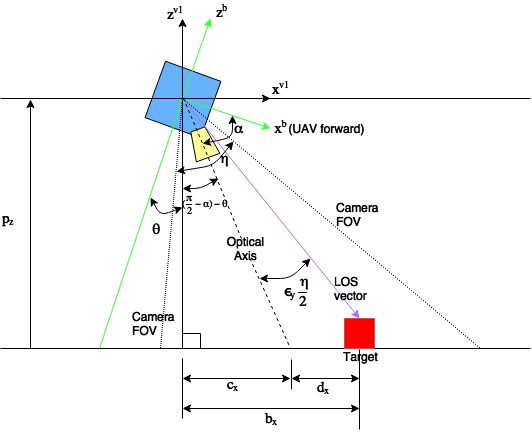
\includegraphics[width=\columnwidth]{side_view_45deg.png}}
	\caption{Side view of the multirotor.}
	\label{side_view}
\end{figure}
The forward motion control strategy is derived from the combination of perspective camera model and multirotor geometry. We assume a calibrated camera and that the controller has access to IMU measurement, that are filtered to provide the orientation of the vehicle. Figure \ref{side_view} depicts the side view of the multirotor. The goal is to compute $d_x$ by subtracting $c_x$ from $b_x$. Let $\eta$ be defined as the camera vertical field of view in radians, $\theta$ be the pitch angle of the multirotor measured by the IMU, and let $p_z$ be the altitude of the multirotor. Also, let $\alpha$ be the angle from $x^b$ to the optical axis of the camera. Notice that the value of $\alpha$ varies depending on how the camera is mounted. Then,

\begin{equation}
c_x=p_z\tan((\frac{\pi}{2}-\alpha)-\theta),
\label{eq4}
\end{equation}
and 

\begin{equation}
b_x=p_z\tan((\frac{\pi}{2}-\alpha)-\theta-\epsilon_y\frac{\eta}{2}),
\label{eq6}
\end{equation} where $\epsilon_y$ is normalized target vertical location in the image, and multiplying $\epsilon_y$ by $\frac{\eta}{2}$ converts the units from normalized image coordinates to radians. Thus, 

\begin{equation}
d_x=b_x-c_x
\label{eq7}
\end{equation} which is the distance that the multirotor has to move along the $x^{v1}$ axis to place the target on the optical axis. This $d_x$ may be broken down into east and north components using the heading of the multirotor. These components are added to the current multirotor east and north positions and sent to the autopilot position controller.


\subsection{Yaw motion control}
In order to compensate the movement of a target that moves horizontally in the image, it is more suitable to do so by a yaw motion of the multirotor than by translating the multirotor sideways. The basic idea of yaw motion control is that if the line of sight (LOS) vector in $\mathcal{F}^o$ is transformed into $\mathcal{F}^{v1}$, the yaw rate command can be found with a proper scale factor. Let 
\begin{equation}
\mathbf{\ell^o}=[\epsilon_x^o, \epsilon_y^o, 1]^\top
\label{eq8}
\end{equation} where $\ell^o$ is the normalized line of sight vector in $\mathcal{F}^o$ and its third element, 1, indicates the focal length of the camera in the normalized image. By applying sequential transformations to $\ell^o$, we get

\begin{equation}
\mathbf{\ell^{v1}}=R^{v1}_b(\phi,\theta)R^b_c(\alpha)R^c_o\ell^o=[\ell^{v1}_x, \ell^{v1}_y, \ell^{v1}_z]^\top
\label{eq9}
\end{equation} where the only second element $\ell^{v1}_y$ matters for yaw motion. It is worth noting that $R^b_c$ is a matrix with fixed values depending on how the camera is mounted with respect to $\mathcal{F}^b$ and that $R^{v1}_b$ requires the roll and pitch angles of the multirotor. Then the yaw rate command $\omega_z$ can be computed as 

\begin{equation}
\omega_z=\gamma \ell^{v1}_y,
\label{eq10}
\end{equation} where $\gamma>0$ is a control gain.


\end{document}